\documentclass[xcolor={usenames,x11names},compress]{beamer}
% Otherwise use xcolor=x11names

%% General document %%%%%%%%%%%%%%%%%%%%%%%%%%%%%%%%%%
\usepackage{graphicx}
\graphicspath{{graphics/}}

% \usepackage{tikz}
% \usetikzlibrary{decorations.pathreplacing}
% \tikzstyle{every picture}+=[remember picture]

\usepackage{color,colortbl}
\input{inputs/rgb}

\usepackage{animate}

% \usepackage[table]{xcolor}
  \usepackage{multirow}


%%%%%%%%%%%%%%%%%%%%%%%%%%%%%%%%%%%%%%%%%%%%%%%%%%%%%%

%% Beamer Layout %%%%%%%%%%%%%%%%%%%%%%%%%%%%%%%%%%

\usetheme{Madrid}
\usecolortheme{seahorse}

\setbeamertemplate{headline}{}
\title{Modelling Global Change Biology}
\author{Samraat Pawar}

\setbeamertemplate{footline}
{
  \leavevmode%
  \hbox{%
%   \begin{beamercolorbox}[wd=.4\paperwidth,ht=2.25ex,dp=1ex,center]{author in 
% head/foot}%
%     \usebeamerfont{author in head/foot}\insertshortauthor
%   \end{beamercolorbox}%
  \begin{beamercolorbox}[wd=.93\paperwidth,ht=2.25ex,dp=1ex,left]{title in 
head/foot}%
    \usebeamerfont{title in head/foot}\insertshorttitle\hspace*{0em}
    --
    \usebeamerfont{author in head/foot}\insertshortauthor

  \end{beamercolorbox}}%
  \begin{beamercolorbox}[wd=.07\paperwidth,ht=2.25ex,dp=1ex,center]{}
     \insertframenumber{} / \inserttotalframenumber\hspace*{1ex}
%       \insertframenumber{}
  \end{beamercolorbox}

%   \vskip0pt%
}

% \useoutertheme[subsection=false,shadow]{miniframes}
\useinnertheme{default}
\usefonttheme{serif}
\usepackage{palatino}

\setbeamerfont{title like}{shape=\scshape}
\setbeamerfont{frametitle}{shape=\scshape, series = \bfseries}
\setbeamertemplate{frametitle}[default][center]
\setbeamertemplate{note page}[plain]

% \setbeamercolor*{lower separation line head}{bg=DeepSkyBlue4} 
% \setbeamercolor*{normal text}{fg=black,bg=white} 
% \setbeamercolor*{alerted text}{fg=red} 
% \setbeamercolor*{example text}{fg=black} 
% \setbeamercolor*{structure}{fg=black}
 
% \setbeamercolor*{palette tertiary}{fg=black,bg=black!10} 
% \setbeamercolor*{palette quaternary}{fg=black,bg=black!10} 

\renewcommand{\(}{\begin{columns}}
\renewcommand{\)}{\end{columns}}
\newcommand{\<}[1]{\begin{column}{#1}}
\renewcommand{\>}{\end{column}}

\def\signed #1{{\leavevmode\unskip\nobreak\hfil\penalty50\hskip2em
  \hbox{}\nobreak\hfil(#1)%
  \parfillskip=0pt \finalhyphendemerits=0 \endgraf}}

\newsavebox\mybox
\newenvironment{aquote}[1]
  {\savebox\mybox{#1}\begin{quote}}
  {\signed{\usebox\mybox}\end{quote}}
  
%%%%%%%%%%%%%%%%%%%%%%%%%%%%%%%%%%%%%%%%%%%%%%%%%%%%

\begin{document}

%%%%%%%%%%%%%%%%%%%%%%%%%%%%%%%%%%%%%%%%%%%%%%%%%%%%%%
\begin{frame}[plain]

\title{Modelling Approaches in Global Change Biology}
\vspace{12pt}
\subtitle{Global Change Biology}
\author{
	Samraat Pawar\\
	\vspace{10pt}
	{\it Imperial College London,\\
	\vspace{5pt}
	Silwood Park}\\
	\vspace{20pt}
  \centering
  \includegraphics[height = .3in]{Imperial_Color1.pdf}
}
 
\titlepage
\end{frame}

%%%%%%%%%%%%%%%%%%%%%%%%%%%%%%%%%%%%%%%%%%%%%%%%%%%%%%
% \section{\scshape Introduction}
% \subsection{}
%%%%%%%%%%%%%%%%%%%%%%%%%%%%%%%%%%%%%%%%%%%%%%%%%%%%%%

%%%%%%%%%%%%%%%%%%%%%%%%%%%%%%%%%%%%%%%%%%%%%%%%%%%%%%
\begin{frame}{Outline}
  \begin{itemize}\setlength{\itemindent}{0em}\itemsep12pt

    \item A primer on modelling (philosophy) 

    \item Key examples of Global Change Biology models/modelling
    \begin{itemize}
        \item Fisheries and over-harvesting 
        \begin{itemize}
          \item Importance of body size and metabolic scaling
        \end{itemize}        
        \item  Carbon cycle and warming
        \begin{itemize}
          \item Importance of thermal physiology
        \end{itemize}        
      \end{itemize}
    
      \item Summary and Readings
    \end{itemize}  

\end{frame}

%%%%%%%%%%%%%%%%%%%%%%%%%%%%%%%%%%%%%%%%%%%%%%%%%%%%%%
\begin{frame}[plain]{}
  
\begin{center}
  {\LARGE \bf A primer on modelling (philosophy)}
\end{center}  

\end{frame}


%%%%%%%%%%%%%%%%%%%%%%%%%%%%%%%%%%%%%%%%%%%%%%%%%%%%%%
\begin{frame}{Modelling in Global Change Biology}

	\begin{center}

    \it What does ``modelling'' mean to you?\\
    \vspace{20pt}
    \pause 
    Caricature of a phenomenon that captures its essence \\ (the model's output reproduces/emulates the phenomenon)
		
  \end{center}
\end{frame}
  
%%%%%%%%%%%%%%%%%%%%%%%%%%%%%%%%%%%%%%%%%%%%%%%%%%%%%%
\begin{frame}{Why use models (Mathematical or not)?}

  \begin{columns}[c]
    \column{2.3in}
    \includegraphics[width=\textwidth]{Reef.jpg}
    \column{2.3in}
    \includegraphics[width=\textwidth]{Forest.jpg}
  \end{columns}

  \centering
  {\it Answer in the context of Global Change Biology}

  \pause

  \begin{itemize}[<+->] \itemsep4pt
  
      \item To understand/explain an observed phenomenon     

      \item To develop accurate predictions of an observed phenomenon in the future    
      
      \item To find out what is important to know in an otherwise complex system
      (cannot measure and monitor everything!)
    
  \end{itemize}

\end{frame}


%%%%%%%%%%%%%%%%%%%%%%%%%%%%%%%%%%%%%%%%%%%%%%%%%%%%%%
\begin{frame}{How to build 'em?}

\begin{columns}[c]
  \column{2.3in}
    \includegraphics[width=\textwidth]{Reef.jpg}
  \column{2.3in}
    \includegraphics[width=\textwidth]{Forest.jpg}
  \end{columns}

  \begin{center}
    {\it Essentially, all models are wrong, but some are useful}\\--- 
    {\small George Box (1987) (British Mathematician)}
  \end{center}

  \pause
  \begin{itemize}[<+->] \itemsep6pt
    \item ``{\it All models are wrong}'' --- every model is a 
      simplification of reality (e.g., the frictionless pendulum!)

    \item ``{\it But some are useful}'' --- the appropriately simplistic 
      ones can ({\it sufficiently}) explain and predict phenomena
  \end{itemize}

\end{frame}


 %%%%%%%%%%%%%%%%%%%%%%%%%%%%%%%%%%%%%%%%%%%%%%%%%%%%%%
 \begin{frame}{Two types of models}

	\begin{itemize}[<+->]\itemsep20pt

		\item {\it Mechanistic models} aim to explain the PROCESSES or
		MECHANISMS underlying PATTERNS or PHENOMENA in empirical data 
		\begin{itemize}
			\item These models have a THEORETICAL BASIS
		\end{itemize}
 
		\item {\it Empirical/Phenomenological models} establish the existence of
		STATISTICALLY SIGNIFICANT, NON-RANDOM PATTERNS or PHENOMENA in empirical
		data 
		\begin{itemize}
			\item They make no assumptions about the processes or mechanisms that generate the patterns
			\item That is, these models lack a THEORETICAL BASIS
		\end{itemize}
			
	  \end{itemize}
 
 \end{frame}
 
%%%%%%%%%%%%%%%%%%%%%%%%%%%%%%%%%%%%%%%%%%%%%%%%%%%%%%
\begin{frame}{Mechanistic vs. Phenomenological models}

\begin{center}
		\includegraphics[width=.7\textwidth]{graphics/L-H_cycle.png}\\
		{\it \tiny source: \url{https://www.cds.caltech.edu/~murray/amwiki/images/8/8f/LHgraph.gif}}
\end{center}
\pause
\begin{itemize}[<+->] \itemsep6pt

	\item {\bf Mechanistic model}: \it The Lynx-Hare Cycle is driven by density-dependent population growth in hares

	\item {\bf Phenomenological model}: \it The Lynx and Hare Cycles have a significant asynchrony (period shift) of x years

\end{itemize}

 \end{frame}
 
 %%%%%%%%%%%%%%%%%%%%%%%%%%%%%%%%%%%%%%%%%%%%%%%%%%%%%%
\begin{frame}{Mechanistic vs. Phenomenological models}

	\begin{itemize}[<+->]\itemsep10pt
		\item {\it It's not really one vs. the other}; Both types of models play a role in science (and Biology)
		\item Phenomenological model-fitting reveals patterns in data that generate HYPOTHESES 
 		\begin{itemize}
			\item These can be tested using further models
			\item Example: {\it Whether} climatic temperature affects the Lynx-Hare cycle (using Generalized Linear Model-fitting)
		\end{itemize} 

		\item Mechanistic model-fitting {\it tries} to validate a mechanistic model that can explain the observed phenomenological pattern and generate MORE ACCURATE, MECHANISTIC HYPOTHESES
		\begin{itemize}
			\item Example: {\it How} climatic temperature {\it drives} the Lynx-Hare cycle
		\end{itemize} 
		\item \it Ultimately, successful, EMPIRICALLY-GROUNDED mechanistic models are the best path towards a THEORY in any scientific discipline (including ecology and evolution)  
	  \end{itemize}
 
 
 \end{frame}

  %%%%%%%%%%%%%%%%%%%%%%%%%%%%%%%%%%%%%%%%%%%%%%%%%%%%%%
\begin{frame}{Mechanistic vs. Phenomenological models}
	 
  \begin{center}
	  \includegraphics[width=\textwidth]{Mechanisms.pdf}
  \end{center} 
 
 \end{frame}

 %%%%%%%%%%%%%%%%%%%%%%%%%%%%%%%%%%%%%%%%%%%%%%%%%%%%%%
\begin{frame}{How to build models --- {\it the} recipe}

  \begin{columns}[c]
    \column{2.3in}
    \includegraphics[width=\textwidth]{Reef.jpg}
    \column{2.3in}
    \includegraphics[width=\textwidth]{Forest.jpg}
  \end{columns}

  \begin{itemize} \itemsep4pt
    \item Build competing models (not just one) --- can be 
      increasingly complex versions of the same basic one
      \pause
    \item Then use Occam's razor ({\it lex parsimoniae}) \pause --- 
      select the competing model with the fewest assumptions (usually, 
      least complexity) \pause (remember model simplification from your R \& Stats weeks! )
  \end{itemize}

  \pause
  Understanding fundamental mechanisms (friction, force) makes life (and       
  modelling) easier (ask any physicist!) \pause --- {\it \bf Mechanistic       
  models!}                                                                     

\end{frame}

%%%%%%%%%%%%%%%%%%%%%%%%%%%%%%%%%%%%%%%%%%%%%%%%%%%%%%
\begin{frame}{A modified recipe for biological modelling}

  \begin{itemize}[<+->] \itemsep6pt
    \item Use knowledge of biological {\it mechanisms} to construct models
    \item But start at the right level of organization! 
      \begin{center}
	\includegraphics[width=.6\textwidth]{Mechanisms.pdf}
      \end{center} 
    \item See if the models ``agree well'' with data
    \item Whichever model ``agrees best'' is most likely to have the right 
      mechanisms --- the one that's best for predictions (e.g., population 
      cycles), estimating rates (e.g., growth rates), etc.
    % \item Of course, {\it model selection} using Occam's Razor will be 
    %   necessary
  \end{itemize}

\end{frame}

%%%%%%%%%%%%%%%%%%%%%%%%%%%%%%%%%%%%%%%%%%%%%%%%%%%%%%
\begin{frame}[plain]{}

  \centering

  {\LARGE \bf Fisheries (importance of Body Size)}\\
  \vspace{10pt}
  \includegraphics[width=.7\textwidth]{Pieter_Fish.jpg}

  \vspace{4pt}

  {\small {\bf \it Big Fish Eat Little Fish}, 1557, Pieter van der Heyden}
\end{frame}

%%%%%%%%%%%%%%%%%%%%%%%%%%%%%%%%%%%%%%%%%%%%%%%%%%%%%%

\begin{frame}{The Goal of Fisheries Modelling}

  \centering 
  \includegraphics[width=.5\textwidth]{Pieter_Fish.jpg}

  \begin{itemize}[<+->] \itemsep4pt
    \item Enable sustainable exploitation ({\it Maximum sustainable yield};  
      MSY)
    \item Accounting for impacts on the wider ecosystem (e.g., non-commercial
      species, potentially of conservation concern)
  \end{itemize}

\end{frame}

%%%%%%%%%%%%%%%%%%%%%%%%%%%%%%%%%%%%%%%%%%%%%%%%%%%%%%
\begin{frame}{Fisheries Modelling Approaches}

  \begin{itemize}[<+->] \itemsep16pt
    \item Single species models

    \item Multi-species models
      \begin{itemize}
	% BGC: Simplify things a bit here.
	%\item Size-spectrum models
	\item Food web models, including the kitchen-sink approach 
      \end{itemize}

    \item Trait-based (species-independent) models
      \begin{itemize}
	\item Size-spectrum models
      \end{itemize}
  \end{itemize}
\end{frame}


%%%%%%%%%%%%%%%%%%%%%%%%%%%%%%%%%%%%%%%%%%%%%%%%%%%%%%
%BGC
\begin{frame}{Single-species fisheries models}

  \begin{itemize}[<+->] \itemsep6pt
    \item Single species models focus on the population dynamics of
      just one species 
    \item There are many different models
    \item A classical one: the Ricker model
      \begin{equation} 
	N_{t+1} = N_t \, e^{r\left(1-\frac{N_t}{K}\right)} 
      \end{equation} 
    \item There are many others (e.g., Beverton-Holt)
    \item \textit{But what of the effect of age, or size?}
  \end{itemize}
\end{frame}


%%%%%%%%%%%%%%%%%%%%%%%%%%%%%%%%%%%%%%%%%%%%%%%%%%%%%%

\begin{frame}{Single-species fisheries models}

  \begin{itemize}[<+->] \itemsep3pt
    \item In another single-species approach, ``cohort'' (individuals born   
      in a same year), are tracked:                                               
				{\small $$N_{1,t+1} = N_{1,t} \, e^{-(z + F_{1,t})}$$
				$$N_{2,t+1} = N_{2,t} \, e^{-(z + F_{2,t})}$$
				$$ . $$
				$$ . $$
				$$ . $$
				$$ N_{k,t+1} = N_{k,t} \, e^{-(z + F_{k,t})}$$

      $z$: ``Natural mortality'' \\
      $F$: Fishing mortality \\
      $k$: Number of cohorts }
    \item $z$ includes mortality due to predation, competition,    
      etc. in a single term (the rest of the ecosystem is a \textit{black box}) 
    \item \textit{Should $z$ be dependent on age or size?} \pause Most likely!
  \end{itemize}

\end{frame}

%%%%%%%%%%%%%%%%%%%%%%%%%%%%%%%%%%%%%%%%%%%%%%%%%%%%%%
\begin{frame}{Single-species fisheries models}

  \textit{Pros and cons of single-species fisheries models}
  \begin{itemize} [<+->]\itemsep6pt
    \item[+] Can include very detailed information on a species, assuming you
      have the data

      \item[+] We know these models well, and have been using them in management
      for a long time

      \item[-] No real idea of the effect of fishing on the wider community
      (e.g., rare species) or on habitats

      \item[-] No species interactions (e.g., cannot capture trophic cascades)

    \end{itemize}
  \vspace{10pt}
  \pause
  \textit{Which goals can we achieve with these models?} 
  \begin{itemize} [<+->]
    \item MSY? -- Perhaps, but if each species has its on MSY, what happens then?
    \item What about the wider ecosystem? Non-target species (fisheries ``by-catches'')?
\end{itemize}
\end{frame}

%%%%%%%%%%%%%%%%%%%%%%%%%%%%%%%%%%%%%%%%%%%%%%%%%%%%%%
\begin{frame}{Multi-species fisheries models}

  \pause
  $\frac{dx_{i}}{dt} =  x_{i}\left[g(\cdot) - \sum_{j\in con(i)}\boxed 
    {\alpha_{ji}}f(\cdot)x_{j} + \sum_{k\in res(i)}\varepsilon_{ik} \boxed 
    {\alpha_{ik}}f(\cdot)x_{k} \right]$
  \vspace{10pt}
  \centering
  \begin{columns}[c]
    \column{1.7in}
    \centering
    \includegraphics[width=1.5in]{graphics/FoodWeb.pdf}
    \column{3.2in}
    \begin{itemize}\setlength{\itemindent}{0em} \itemsep10pt
	\pause
      \item Such models are necessarily more complex
      \item They account for species interactions 
      \item They account for dynamics like trophic cascades 
      \item These include the kitchen sink approach such as \textit{Ecopath    
	  with Ecosim} (and \textit{Ecospace}, etc.; developed by UBC, Cefas,           
	\textit{et al.}) and \textit{Atlantis} (developed by Beth Fulton at CSIRO)    
    \end{itemize}
  \end{columns}

\end{frame}

%%%%%%%%%%%%%%%%%%%%%%%%%%%%%%%%%%%%%%%%%%%%%%%%%%%%%%
\begin{frame}{Multi-species fisheries models}

  \textit{Pros and cons of multi-species fisheries models}

  \begin{itemize} [<+->]\itemsep6pt
    \item[+] Can account for species interactions 

    \item[+] Estimate wider ecosystem impacts 
      \begin{itemize}
        \item Effects on non-target species
        \item Effects on overall quality of the ecosystem
      \end{itemize}
    \item[+] Project long-term scenarios

      \item[-] very ambitious, can become very complex, and as a result
      \begin{itemize}
	      \item Become black boxes (who knows what's going on in the model?)
	      \item Require a \textit{lot} of data, which are not always available
      \end{itemize}
      \item [-] Their complexity means that they can fail miserably (can't even predict next year's catch)
  \end{itemize}

\end{frame}

%%%%%%%%%%%%%%%%%%%%%%%%%%%%%%%%%%%%%%%%%%%%%%%%%%%%%%
\begin{frame}{Multi-species fisheries models}

  \begin{itemize}[<+->]\itemsep10pt
    \item We can {\it potentially} better meet sustainable fisheries objectives with multi-species fisheries models
    \item Because we can capture the wider ecosystem effects of fisheries with them
    \item But data, parameters, details\ldots
    \item These models are necessarily more complex because they needed parameterisation of species interaction (consumption) rates
    \item How do we predict / parameterise the interaction rates between myriad species?
    \item Mechanistic Modelling to the rescue
    \begin{itemize}
      \item Using metabolic (size) scaling (Importance of body size)
    \end{itemize}
  \end{itemize}
  
  \end{frame}

%%%%%%%%%%%%%%%%%%%%%%%%%%%%%%%%%%%%%%%%%%%%%%%%%%%%%
\begin{frame}{Mechanistic Fisheries models: Using size scaling}
  \pause
  \begin{itemize}
    \item Metabolic rate: Rate of individual's energy use (watts, J/s, kcal/s)
    \item Metabolic rate in the resting state ($B$) sets the ``pace of life''
      \pause
    \item B increases with body size ($M$) as a ``power-law'':

  \begin{columns}[c]
	  \column{2.5in}\centering
	  $B = B_0 \, M^{b}$ (where $b = 0.75$ )\\
	  \includegraphics[width=0.9\textwidth]{MetabScaling.jpg} \\ (Kleiber's Law)
	\column{2.5in}\centering
	\pause
	\includegraphics[width=0.45\textwidth]{fester.jpg}
	\begin{itemize}
	  \item {\it Your wattage is $\sim$75W (unless you are sleeping!)}
	\end{itemize}
      \end{columns}
  \end{itemize}

\end{frame}

%%%%%%%%%%%%%%%%%%%%%%%%%%%%%%%%%%%%%%%%%%%%%%%%%%%%%%
\begin{frame}{Using size scaling}

  \begin{columns}[c]
    \column{0.45\textwidth}\centering
    Because
    \vspace{10pt}\\
    \includegraphics[width=\textwidth]{MetabScaling.jpg} 
    \column{0.55\textwidth}\centering
    \pause
    Therefore,\\ \pause
    \includegraphics[width=.9\textwidth]{graphics/DimRes1.pdf}
    Size predicts interaction rates ({\it voila!})
  \end{columns}

\end{frame}

%%%%%%%%%%%%%%%%%%%%%%%%%%%%%%%%%%%%%%%%%%%%%%%%%%%%
\begin{frame}{Using Size scaling}

\begin{columns}
  \column{0.6\textwidth}\centering
    \includegraphics[width=.9\textwidth]{DimRes1.pdf}
  \column{0.4\textwidth}\centering
    \begin{itemize}\setlength{\itemindent}{0em}
      \item Size predicts interaction rates (consumption rates)
      \item 3$D$ consumption rates scale differently than 2$D$
      % \item Search rates drive differences in consumption rate scaling
    \end{itemize}
    \vspace{6pt}
    \includegraphics[width=.9\textwidth]{Dimensionality.pdf}\\
    {\tiny Pawar et al Nature 2012}
\end{columns}

\end{frame}

%%%%%%%%%%%%%%%%%%%%%%%%%%%%%%%%%%%%%%%%%%%%%%%%%%%%%%
\begin{frame}{Multi-species fisheries models}

  \begin{columns}[c]
    \column{0.25\textwidth}\centering
      \includegraphics[width=\textwidth]{graphics/FoodWeb.pdf}
    \column{0.75\textwidth}\centering
    \includegraphics[width=.6\textwidth]{DimRes1.pdf}
  \end{columns}

  \vspace{10pt}

  \begin{itemize}\setlength{\itemindent}{0em} \itemsep10pt
        \item Metabolic (size) scaling can help {\it mechanistically  parameterise} (provide values for the $\alpha$'s in the multi-species model) 
  \end{itemize}

\end{frame}

%%%%%%%%%%%%%%%%%%%%%%%%%%%%%%%%%%%%%%%%%%%%%%%%%%%%%%
\begin{frame}{A compromise: Size-spectrum models}

  \begin{itemize}
     \item Size-spectrum models try to capture energy/biomass flows across trophic levels in  marine food webs {\it without worrying about specific species interactions}
     
     \begin{center}
        \includegraphics[width=.35\textwidth]{size_spectrum.jpg} 
     \end{center}

     \item All that matters in these models is size, irrespective of species identity
     
     \item Thus they are essentially ``trait-based'' (species-independent) models

  \end{itemize}

\end{frame}

%%%%%%%%%%%%%%%%%%%%%%%%%%%%%%%%%%%%%%%%%%%%%%%%%%%%%%
\begin{frame}{Size-Specturm Fisheries models}

  \begin{itemize}\itemsep10pt
     
    \item They can capture effects such as trophic cascades without the underlying complexity of the food web

    \item These models can work quite well for mid-term forecasting (better than single-species, not as good as multi-species models - when the latter are actually working well) 
    
    \item But the jury is still out on effective size-spectrum models really are (species interactions do matter at some level)

  \end{itemize}

\end{frame}

%%%%%%%%%%%%%%%%%%%%%%%%%%%%%%%%%%%%%%%%%%%%%%%%%%%%%%
\begin{frame}{Size-spectrum Fisheries models: mechanistic basis}

  \begin{itemize}
    \item These models use ``Damuth's law'' to estimate the ``size spectrum'' of a community
     
    \centering 
    
    \includegraphics[width=.65\textwidth]{Damuth.png}

  \end{itemize}

\end{frame}

%%%%%%%%%%%%%%%%%%%%%%%%%%%%%%%%%%%%%%%%%%%%%%%%%%%%%%
\begin{frame}{The mechanistic basis of Size-specturm Models}

  \begin{columns}[c]
    \column{2.4in}\centering
    Resting metabolic rate (watts),\\ 
    $B = B_0 M^{0.75}$\\
    {\small (''Kleiber's Law``: Metabolic rate increases {\it allometrically} with size)}\\[10pt]
    % \vspace{10pt}
    \includegraphics[width=2.2in]{MetabScaling.jpg} 
    \column{2.4in}\centering
    \pause
    Therefore,\\ 
    $r_\text{max} = r_0 M^{-0.25} $\\
    (Population growth rate declines {\it allometrically} with body size)\\[10pt]
    % \vspace{20pt}
    \includegraphics[width=2.2in]{r_max.pdf}
  \end{columns}
\pause   
\end{frame}

%%%%%%%%%%%%%%%%%%%%%%%%%%%%%%%%%%%%%%%%%%%%%%%%%%%%%
\begin{frame}{The mechanistic basis of Size-specturm Models}

  \begin{itemize} \itemsep10pt
    \item So in general, larger animals and plants have relatively less power to crank out offspring

  \begin{columns}[c]
    \column{2.5in}\centering
    \centering
    \includegraphics[width=0.8\textwidth]{r_max.pdf}
    \column{2.5in}\centering
    \pause
    \includegraphics[width=0.8\textwidth]{Elephants.jpg}
  \end{columns}

    \item {\it This} is why smaller organisms typically show stronger exponential growth than larger ones!
  \end{itemize}

\end{frame}

%%%%%%%%%%%%%%%%%%%%%%%%%%%%%%%%%%%%%%%%%%%%%%%%%%%%%%
\begin{frame}{The mechanistic basis of Size-specturm Models}

  \begin{itemize}
    \item And, assuming sufficient energy supply to all species, population density will scale negatively with body size ({\it Damuth's law})

    \begin{center}
      \includegraphics[width=.5\textwidth]{Damuth.png} 
    \end{center}
 \vspace{-10pt}

  \item So big animals and plants are rarer 
   \item Carnivores of a given size are rarer than herbivores of the same size  because less energy is available higher up in food chains

  \end{itemize}

\end{frame}

%%%%%%%%%%%%%%%%%%%%%%%%%%%%%%%%%%%%%%%%%%%%%%%%%%%%%%
\begin{frame}[plain]{}
  \centering

  {\Large \bf Global Warming and Carbon Balance (importance of Thermal Physiology)}\\
  \vspace{10pt}
  \includegraphics[width=.7\textwidth]{800.jpg}

  \vspace{4pt}

  {\small {\bf \it The world's getting warmer}}
\end{frame}


%%%%%%%%%%%%%%%%%%%%%%%%%%%%%%%%%%%%%%%%%%%%%%%%%%%%%%
\begin{frame}{Earth's Carbon Cycle}

  \centering
  \includegraphics[width=.7\textwidth]{graphics/Carbon_cycle.jpg}\\
\vspace{-8pt}
{\tiny \url{https://en.wikipedia.org/wiki/Carbon_cycle}}
\end{frame}

%%%%%%%%%%%%%%%%%%%%%%%%%%%%%%%%%%%%%%%%%%%%%%%%%%%%%%
\begin{frame}{Mathematically Modelling the Carbon Cycle}

\begin{itemize}[<+->]\itemsep10pt
  \item Ecosystem-scale models 
    \begin{itemize}
      \item Seek to model the cycling of carbon within specific ecosystems (e.g, in pond, lake, ocean, soil, grassland, forest) 
      \item Often focus on net Greenhouse Gas (GHG) emission vs sequestration (absorbtion / storage)
      \item They often ignore feedbacks between the biological (e.g., the food web) and physical (e.g., water or soil chemistry) components of the ecosystem
    \end{itemize}
    \item Global-scale models
    \begin{itemize}
      \item Seek to model the cycling of carbon {\it across} ecosystems 
      \item Typically, they are global- (Earth-) scale models 
      \item They typically include feedbacks between the biological and physical components of the Globe (therefore, AKA ``Earth system models, or ESMs'') 
    \end{itemize}
    \item \it We will focus on Ecosystem-scale models in this lecture
\end{itemize}

\end{frame}

%%%%%%%%%%%%%%%%%%%%%%%%%%%%%%%%%%%%%%%%%%%%%%%%%%%%%%
\begin{frame}{Ecosystem Scale Carbon Cycle Models}

  \begin{itemize}[<+->]\itemsep0pt
    \item Compartment-based: divide the ecosystem into functional compartments and model carbon flows/fluxes between/through them\\[10pt]
    \centering
    \includegraphics[width=.5\textwidth]{EltonFW.pdf}
    \item They typically assume that abundances in the different compartments are not fluctuating (steady-state assumption)  

  \end{itemize}
  
\end{frame}

%%%%%%%%%%%%%%%%%%%%%%%%%%%%%%%%%%%%%%%%%%%%%%%%%%%%%%
\begin{frame}{Ecosystem-Scale Carbon Cycle Models}

  \begin{itemize}[<+->]\itemsep10pt
    \item Food web-based: explicitly model the flows of carbon through the trophic network\\[10pt]
    \centering
    \includegraphics[width=.35\textwidth]{FoodWeb.pdf}
  \item They may or may not make a steady-state assumption

  \end{itemize}
  
\end{frame}

%%%%%%%%%%%%%%%%%%%%%%%%%%%%%%%%%%%%%%%%%%%%%%%%%%%%%%
\begin{frame}{Multi-species fisheries models}

  \textit{Pros and cons of the different Ecosystem-scale Carbon cycle models}

  \begin{itemize} [<+->]\itemsep10pt
    \item Compartment-based models

    \begin{itemize} 
      \item[+] Relatively simple, require less parameterisation
      \item[-] Assume steady state, so cannot capture dynamics, or include effects of changing species composition (e.g., driven by climate change)
    \end{itemize}
    
    \item Food web-based models
    \begin{itemize} 
      \item[+] Can provide predictions based on a steady state assumption, or can model changes in dynamics/abundances of component populations driven by factors such as climate change
      \item[+] So can potentially predict future trends in ecosystem carbon cycling
      \item[-] Difficult to parameterise (same issues as multi-species fisheries models, and same potential solution, using metabolic scaling)
    \end{itemize}
  \end{itemize}

\end{frame}

%%%%%%%%%%%%%%%%%%%%%%%%%%%%%%%%%%%%%%%%%%%%%%%%%%%%%%
\begin{frame}{Including climatic warming into Ecosystem-scale Carbon Cycle models}

  \begin{itemize}[<+->]\setlength{\itemindent}{0em}\itemsep2pt
    \item Earth's Carbon Cycle is {\it inevitably} temperature-dependent

  \begin{center}
    \includegraphics[width=0.8\textwidth]{Bar-on_et_al.pdf}\\
    {\tiny Bar-On et al, ``The Biomass Distribution on Earth'' PNAS 2018}
  \end{center}\par

    \item Metabolic rates of the {\it vast majority} of life depend directly on environmental temperature
    \item The rest, endotherms, also depend indirectly on temperature (e.g., they eat ectotherms, such as rabbit eating grass)
  \end{itemize}

  \end{frame}

% %%%%%%%%%%%%%%%%%%%%%%%%%%%%%%%%%%%%%%%%%%%%%%%%%%%%%
\begin{frame}{The world's getting warmer (duh!)}

  \centering
  \includegraphics[width=4in]{Warming.png}

\end{frame}

% %%%%%%%%%%%%%%%%%%%%%%%%%%%%%%%%%%%%%%%%%%%%%%%%%%%%%
% \begin{frame}{Thermal fluctuations are also predicted to increase}

%   \centering
%   \includegraphics[width=2.5in]{graphics/Fluctuations.jpg}\\
%   \vspace{5pt}
%   \centering
%   \includegraphics[width=4.3in]{graphics/ClimFluctHot.jpg}

% \end{frame}

%%%%%%%%%%%%%%%%%%%%%%%%%%%%%%%%%%%%%%%%%%%%%%%%%%%%%%
\begin{frame}{Modelling effects of climatic warming on the Carbon Cycle}

  \begin{itemize}[<+->] \itemsep6pt
			\item We can understand effects on carbon balance by modelling:
      \begin{itemize} \itemsep4pt
				\item Carbon Use Efficiency (CUE) --- quantifies organismal growth efficiency and ecosystem productivity potential
					$$\textrm{CUE}  = 1 - \frac{R}{P_{\textrm{gross}}}$$
				\item Net carbon flux (exchange) --- the rate of organismal and 
				ecosystem carbon gain or loss due to metabolism
				$$\textrm{Net carbon flux} = P_{\textrm{net}} - R$$
			\end{itemize}
  \end{itemize}
  $R$: Respiration rate (plants + heterotrophs -- microbes and animals)\\
  $P_{\text{gross}}$: (Diurnal) Gross photosynthesis rate \\ 
  $P_{\text{net}}$: Diurnal net photosynthesis rate (difference between $P_\text{gross}$ and diurnal respiration rate of plants)

\end{frame}

 %%%%%%%%%%%%%%%%%%%%%%%%%%%%%%%%%%%%%%%%%%%%%%%%%%%%%
\begin{frame}{Ecosystem-scale Carbon cycle Models: The importance of thermal physiology}
      
  \begin{columns}[c]
    \column{2.1in}
    \pause
    \includegraphics[width=\textwidth]{graphics/Photobacterium.pdf}\\
    {\scriptsize (J H van't Hoff 1884, S Arrhenius 1889)}
    \pause
    \column{2.7in}
    $B = B_0 \boxed {e^{-\frac{E}{kT}}}f(T,T_{pk},E_D)$\\
    \vspace{6pt}
    \raggedright{\footnotesize $T$ = temperature (K)\\
    $B$ = The metabolic (e.g., Photosynthesis, Respiration) rate \\   
    $B_0$ = A ``normalization'' constant (may include effect of body size) \\   
    $k$ = Boltzmann constant (eV K$^{-1}$)\\
    $E$ = Activation energy (eV) (thermal sensitivity)\\
    $T_{pk}$ = Temperature of peak performance\\
    $E_D$ = Deactivation energy (eV)}
  \end{columns}

  \pause

  \begin{itemize}\setlength{\itemindent}{0em}

    \item This is very general; key biological rates: Respiration, photosynthesis, consumption rate, growth rate, etc., all depend upon temperature in a similar way (following the above equation)

  \end{itemize} 

\end{frame}

%%%%%%%%%%%%%%%%%%%%%%%%%%%%%%%%%%%%%%%%%%%%%%%%%%%%%%
\begin{frame}{Modelling effects of climatic warming on the Carbon Cycle}
  \begin{itemize}
			\item Ecosystem carbon balance depends on differences in the 
			thermal responses of respiration (which releases carbon) and 
			photosynthesis (which fixes carbon) rates:
  \end{itemize}

  \begin{center} \it
    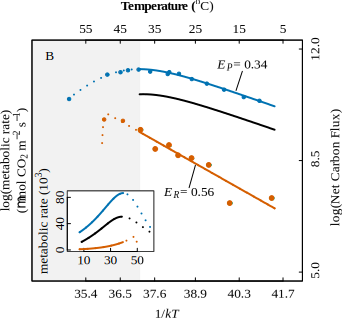
\includegraphics[width=.45\textwidth]{Fig1_IntraspPlotsTerAqInv.pdf}

\pause 
Note that these are Arrhenius plots (temperature axis is inverted)
\end{center}

\end{frame}

%%%%%%%%%%%%%%%%%%%%%%%%%%%%%%%%%%%%%%%%%%%%%%%%%%%%%%
\begin{frame}{Summary}
   
    \begin{itemize}[<+->] \setlength{\itemindent}{0em} \itemsep6pt
  
      \item Mechanistic Modelling is key to {\it predictive} Models in Global Change Biology 
      
      \item Species' body sizes determine their population growth rate and population size
      \begin{itemize}
        \item Therefore size also predicts the robustness to and recovery from perturbations of species' populations in both fisheries and carbon cycle models
      \end{itemize} 

      \item Fisheries Models have historically not been particularly accurate or forward looking (predictive)
        \begin{itemize}
          \item Using metabolic theory to develop more mechanistic. muti-species fisheries  models is necessary (and is a work in progress) 
        \end{itemize}  
        
        \item Metabolic theory can be used to model the balance of  whole-ecosystem respiration and primary production (Ecosystem-scale carbon cycle models)

        \begin{itemize}
          \item Because environmental temperature determines metabolic rate, and most life on earth is ectothermic 
        \end{itemize}  

    \end{itemize}
    
  \end{frame}  

  %%%%%%%%%%%%%%%%%%%%%%%%%%%%%%%%%%%%%%%%%%%%%%%%%%%%%%
\begin{frame}{Readings}

  \begin{enumerate}\itemsep2pt

    \item Brown, J. H.,  et al. Toward a metabolic theory of ecology. Ecology 85, 1771--1789. (2004). 

    \item Dell, A. I. et al. Systematic variation in the temperature dependence
      of physiological and ecological traits. PNAS. 108, 10591--10596. (2011)
    
    \item Sprules, W. G. \& Barth, L. E. Surfing the biomass size spectrum: Some remarks on history, theory, and application. Canadian Journal of Fisheries and Aquatic Sciences vol. 73 477--495 (2016).
    
    \item Schramski, J. R. et al. Metabolic theory predicts whole-ecosystem properties. PNAS 112, 2617--2622. (2015).
    
    \item Yvon-Durocher, G. et al. Reconciling the temperature dependence of respiration across timescales and ecosystem types. Nature 487, 472--476 (2012).

    \item Smith, T.P. et al. Community-level respiration of prokaryotic microbes
    may rise with global warming. Nat. Commun. 10 (1) (2019). 

  \end{enumerate}


\end{frame}

\end{document}
